\documentclass[12pt]{article}

\usepackage[margin=3cm]{geometry}
\usepackage{graphicx}
\usepackage{minted}
\usepackage{pdfpages}
\usepackage{minted}
\usepackage{float}

\author{Pablo Vargas Bermúdez}

\begin{document}

\pagestyle{empty}

\includepdf[pages=-]{Portada}

\section*{Descripción}

\begin{figure}[H]
  \centering
  \includegraphics[width=.5\textwidth]{figures/descripcion.png}
  \caption{Barbero durmiente}
\end{figure}


Realiza una investigación acerca del problema del barbero durmiente,
una vez comprendido realiza un programa que permita mostrar el
funcionamiento de dicho problema mediante los hilos que hemos estado
trabajando.

Realiza un diagrama  UML de las clases que diseñes.

Envía un archivo PDF que contenga una hoja de presentación, la
descripción de la tarea, la investigación realizada, los diagrama UML
y el código fuente del programa que muestra el problema del barbero
durmiente y las capturas de pantalla necesarias donde muestres el
correcto funcionamiento.

\section*{Investigación}

En ciencias de la computación, el problema del barbero durmiente es un
problema de sincronización.

El problema consiste en una barbería en la que trabaja un barbero que
tiene un único sillón de barbero y varias sillas para esperar. Cuando
no hay clientes, el barbero se sienta en una silla y se duerme. Cuando
llega un nuevo cliente, éste o bien despierta al barbero o si el
barbero está afeitando a otro cliente se sienta en una silla (o se va
si todas las sillas están ocupadas por clientes esperando). El
problema consiste en realizar la actividad del barbero sin que ocurran
condiciones de carrera. La solución implica el uso de semáforos y
objetos de exclusión mutua para proteger la sección crítica.

Un semáforo es una variable protegida (o tipo abstracto de datos) que
constituye el método clásico para restringir o permitir el acceso a
recursos compartidos (por ejemplo, un recurso de almacenamiento) en un
entorno de multiprocesamiento. Fueron inventados por Edsger Dijkstra y
se usaron por primera vez en el sistema operativo THEOS.

En electrónica y en programación concurrente, se conoce como condición
de carrera al error que se produce en programas o circuitos lógicos
que no se han construido adecuadamente para su ejecución simultánea
con otros procesos.

\begin{itemize}
\item Barbería con un solo barbero.
\item Una silla de barbero.
\item N sillas para los clientes
\end{itemize}

\section*{Diagrama UML}

\begin{figure}[H]
  \centering
  \includegraphics[width=\textwidth]{figures/UML.png}
  \caption{Diagrama UML}
\end{figure}


\section*{Código}

\inputminted{Java}{BarberoDurmiente.java}

\section*{Ejecución}

\begin{figure}[H]
  \centering
  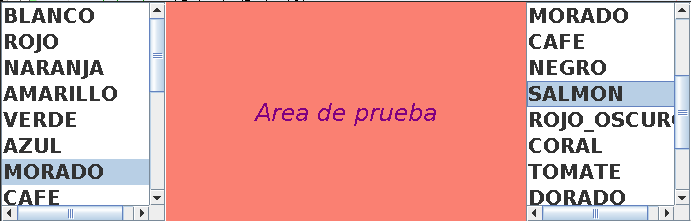
\includegraphics[width=.7\textwidth]{figures/run1.png}
  \caption{Ejecución con N = 5}
\end{figure}

\begin{figure}[H]
  \centering
  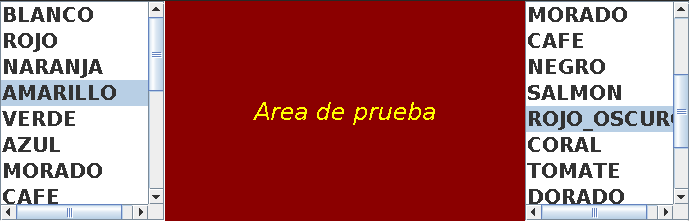
\includegraphics[width=.7\textwidth]{figures/run2.png}
  \caption{Ejecución con N = 10}
\end{figure}

\begin{figure}[H]
  \centering
  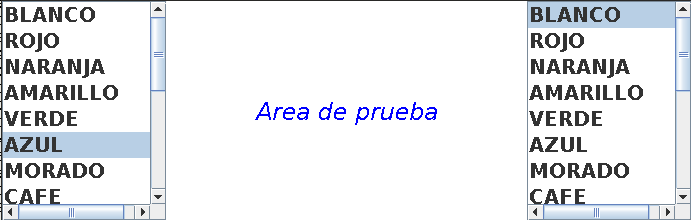
\includegraphics[width=.7\textwidth]{figures/run3.png}
  \caption{Ejecución con N = 15}
\end{figure}

\end{document}
